\section{Abstract}
Hypersonic vehicles demand high performance from every subsystem, with emphasis on a stable propulsion system and material capabilities. This project aims to investigate the feasibility of using a gas-fueled Rotating Detonation Engine (RDE) in a hypersonic vehicle with a cruise Mach of 6.5 at 1500 psf of dynamic pressure, launched on the GO1 platform. It was found that an ethylene fueled RDE, paired with a conical inlet and various cooling systems, is potentially capable of 107 seconds of flight, 45 second of which at cruise velocity. Most notable is a cruise Isp of 2080 seconds, which is substantially higher than conventional scramjet burners. The preliminary design shows that, while an RDE may be feasible for such a mission, extensive fundamental research is required to fully understand the operation of an RDE. A overview of the final design can be seen in Figure \ref{fig:totalIsoView}.

 \begin{figure}[H]
\begin{center}
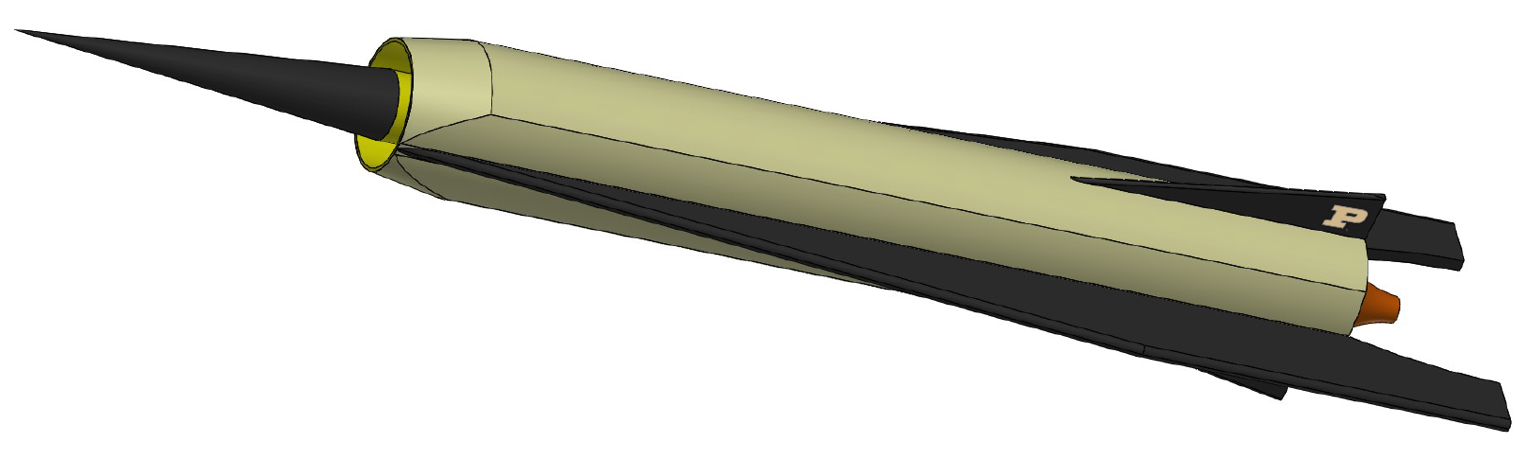
\includegraphics[width=\textwidth]{totalIsoView}
\caption{Overview of Final Design}
\label{fig:totalIsoView}
\end{center}
\end{figure}